% -*- Mode:TeX -*-

%% IMPORTANT: The official thesis specifications are available at:
%%            http://libraries.mit.edu/archives/thesis-specs/
%%
%%            Please verify your thesis' formatting and copyright
%%            assignment before submission.  If you notice any
%%            discrepancies between these templates and the 
%%            MIT Libraries' specs, please let us know
%%            by e-mailing thesis@mit.edu

%% The documentclass options along with the pagestyle can be used to generate
%% a technical report, a draft copy, or a regular thesis.  You may need to
%% re-specify the pagestyle after you \include  cover.tex.  For more
%% information, see the first few lines of mitthesis.cls. 

%\documentclass[12pt,vi,twoside]{mitthesis}
%%
%%  If you want your thesis copyright to you instead of MIT, use the
%%  ``vi'' option, as above.
%%
%\documentclass[12pt,twoside,leftblank]{mitthesis}
%%
%% If you want blank pages before new chapters to be labelled ``This
%% Page Intentionally Left Blank'', use the ``leftblank'' option, as
%% above. 

\documentclass[12pt,twoside]{mitthesis}

\pdfminorversion=7
\usepackage[pdftex]{graphicx}
\graphicspath{{../../../schematics/svg/}{../../../schematics/imagenes/}}
\DeclareGraphicsExtensions{.pdf,.jpeg,.png,.eps}

\usepackage{subfig}

\usepackage{titlesec}
\titleformat{\chapter}[display]
{\normalfont\bfseries}{}{0pt}{\huge}

\usepackage{multirow}
\usepackage{lgrind}
%% These have been added at the request of the MIT Libraries, because
%% some PDF conversions mess up the ligatures.  -LB, 1/22/2014
\usepackage{cmap}
\usepackage[T1]{fontenc}
\pagestyle{plain}

%% This bit allows you to either specify only the files which you wish to
%% process, or `all' to process all files which you \include.
%% Krishna Sethuraman (1990).

% \typein [\files]{Enter file names to process, (chap1,chap2 ...), or `all' to
% process all files:}
% \def\all{all}
% \ifx\files\all \typeout{Including all files.} \else \typeout{Including only \files.} \includeonly{\files} \fi

\begin{document}

% -*-latex-*-
% 
% For questions, comments, concerns or complaints:
% thesis@mit.edu
% 
%
% $Log: cover.tex,v $
% Revision 1.8  2008/05/13 15:02:15  jdreed
% Degree month is June, not May.  Added note about prevdegrees.
% Arthur Smith's title updated
%
% Revision 1.7  2001/02/08 18:53:16  boojum
% changed some \newpages to \cleardoublepages
%
% Revision 1.6  1999/10/21 14:49:31  boojum
% changed comment referring to documentstyle
%
% Revision 1.5  1999/10/21 14:39:04  boojum
% *** empty log message ***
%
% Revision 1.4  1997/04/18  17:54:10  othomas
% added page numbers on abstract and cover, and made 1 abstract
% page the default rather than 2.  (anne hunter tells me this
% is the new institute standard.)
%
% Revision 1.4  1997/04/18  17:54:10  othomas
% added page numbers on abstract and cover, and made 1 abstract
% page the default rather than 2.  (anne hunter tells me this
% is the new institute standard.)
%
% Revision 1.3  93/05/17  17:06:29  starflt
% Added acknowledgements section (suggested by tompalka)
% 
% Revision 1.2  92/04/22  13:13:13  epeisach
% Fixes for 1991 course 6 requirements
% Phrase "and to grant others the right to do so" has been added to 
% permission clause
% Second copy of abstract is not counted as separate pages so numbering works
% out
% 
% Revision 1.1  92/04/22  13:08:20  epeisach

% NOTE:
% These templates make an effort to conform to the MIT Thesis specifications,
% however the specifications can change.  We recommend that you verify the
% layout of your title page with your thesis advisor and/or the MIT 
% Libraries before printing your final copy.
\title{Práctica Profesional Supervisada\\
  \large Reuso Dinámico de Memoria en Convolución 2D Aplicada a Procesamiento de
Imágenes}

\author{Casabella Martín, Sulca Sergio, Vignolles Ivan}
% If you wish to list your previous degrees on the cover page, use the 
% previous degrees command:
%       \prevdegrees{A.A., Harvard University (1985)}
% You can use the \\ command to list multiple previous degrees
%       \prevdegrees{B.S., University of California (1978) \\
%                    S.M., Massachusetts Institute of Technology (1981)}
\department{Escuela de Ingeniería en Computación}

% If the thesis is for two degrees simultaneously, list them both
% separated by \and like this:
% \degree{Doctor of Philosophy \and Master of Science}
\degree{Bachelor of Science in Computer Science and Engineering}

% As of the 2007-08 academic year, valid degree months are September, 
% February, or June.  The default is June.
\degreemonth{Septiembre}
\degreeyear{2018}
\thesisdate{Septiembre, 2018}

%% By default, the thesis will be copyrighted to MIT.  If you need to copyright
%% the thesis to yourself, just specify the `vi' documentclass option.  If for
%% some reason you want to exactly specify the copyright notice text, you can
%% use the \copyrightnoticetext command.  
%\copyrightnoticetext{\copyright IBM, 1990.  Do not open till Xmas.}
\copyrightnoticetext{}

% If there is more than one supervisor, use the \supervisor command
% once for each.
\supervisor{William J. Dally}{Associate Professor}

% This is the department committee chairman, not the thesis committee
% chairman.  You should replace this with your Department's Committee
% Chairman.
\chairman{Arthur C. Smith}{Chairman, Department Committee on Graduate Theses}

% Make the titlepage based on the above information.  If you need
% something special and can't use the standard form, you can specify
% the exact text of the titlepage yourself.  Put it in a titlepage
% environment and leave blank lines where you want vertical space.
% The spaces will be adjusted to fill the entire page.  The dotted
% lines for the signatures are made with the \signature command.
\maketitle

% The abstractpage environment sets up everything on the page except
% the text itself.  The title and other header material are put at the
% top of the page, and the supervisors are listed at the bottom.  A
% new page is begun both before and after.  Of course, an abstract may
% be more than one page itself.  If you need more control over the
% format of the page, you can use the abstract environment, which puts
% the word "Abstract" at the beginning and single spaces its text.

%% You can either \input (*not* \include) your abstract file, or you can put
%% the text of the abstract directly between the \begin{abstractpage} and
%% \end{abstractpage} commands.

% First copy: start a new page, and save the page number.
\cleardoublepage
% Uncomment the next line if you do NOT want a page number on your
% abstract and acknowledgments pages.
% \pagestyle{empty}
\setcounter{savepage}{\thepage}
\begin{abstractpage}
% $Log: abstract.tex,v $
% Revision 1.1  93/05/14  14:56:25  starflt
% Initial revision
% 
% Revision 1.1  90/05/04  10:41:01  lwvanels
% Initial revision
% 
%
%% The text of your abstract and nothing else (other than comments) goes here.
%% It will be single-spaced and the rest of the text that is supposed to go on
%% the abstract page will be generated by the abstractpage environment.  This
%% file should be \input (not \include 'd) from cover.tex.
\section*{\small Objetivo}\label{objetivo_sec}
{\renewcommand\baselinestretch{1}\small
El objetivo de la Práctica Profesional Supervisada, en adelante PPS, es lograr la inserción laboral del alumno en la realidad profesional del país, en el área que mejor responda a sus aspiraciones profesionales e intereses vocacionales, con el propósito de fortalecer su formación académica y de establecer un vínculo que facilite su ingreso como profesional al mercado de trabajo. 
Este proyecto consta en el diseño e implementación en una FPGA (Field Programmable Gate Array) de un sistema destinado al procesamiento digital de imágenes vía hardware. 
Fue desarrollado en la institución Fulgor, bajo la supervisión del Dr.Ing. Ariel
Luis Pola. \par}

\section*{\small Motivación}\label{motiv_sec}
{\renewcommand\baselinestretch{1}\small
El filtrado y procesamiento de imágenes es utilizado en múltiples campos, como la medicina, ingeniería, navegación, aeronáutica, entre otros. En el campo de la inteligencia artificial, área emergente que es de mero interés hoy en día, la convolución en 2D es la operación principal que se realiza durante el feed forward de una CNN (Red neuronal Convolucional). 
Dada su naturaleza, la operación de convolución en 2-D es la más empleada en los algoritmos de procesamiento de imágenes. El paralelismo inherente de algoritmos basados en la convolución es explotado logrando alta performance en estos sistemas que los utilizan.
El uso de Field Programmable Gate Arrays (FPGAs) para implementar este tipo de sistemas, se debe a la ventaja que presentan estos dispositivos en lo que concierne al paralelismo a nivel bit, pixel, vecindad y a nivel tarea, lo incrementa la performance y velocidad de cómputo.
Se presenta una arquitectura para la implementación en hardware de la operación
de convolución 2-D priorizando el uso eficiente de recursos junto con la
escalabilidad del diseño y velocidad de procesamiento. \par}
\end{abstractpage}

% Additional copy: start a new page, and reset the page number.  This way,
% the second copy of the abstract is not counted as separate pages.
% Uncomment the next 6 lines if you need two copies of the abstract
% page.
% \setcounter{page}{\thesavepage}
% \begin{abstractpage}
% % $Log: abstract.tex,v $
% Revision 1.1  93/05/14  14:56:25  starflt
% Initial revision
% 
% Revision 1.1  90/05/04  10:41:01  lwvanels
% Initial revision
% 
%
%% The text of your abstract and nothing else (other than comments) goes here.
%% It will be single-spaced and the rest of the text that is supposed to go on
%% the abstract page will be generated by the abstractpage environment.  This
%% file should be \input (not \include 'd) from cover.tex.
\section*{\small Objetivo}\label{objetivo_sec}
{\renewcommand\baselinestretch{1}\small
El objetivo de la Práctica Profesional Supervisada, en adelante PPS, es lograr la inserción laboral del alumno en la realidad profesional del país, en el área que mejor responda a sus aspiraciones profesionales e intereses vocacionales, con el propósito de fortalecer su formación académica y de establecer un vínculo que facilite su ingreso como profesional al mercado de trabajo. 
Este proyecto consta en el diseño e implementación en una FPGA (Field Programmable Gate Array) de un sistema destinado al procesamiento digital de imágenes vía hardware. 
Fue desarrollado en la institución Fulgor, bajo la supervisión del Dr.Ing. Ariel
Luis Pola. \par}

\section*{\small Motivación}\label{motiv_sec}
{\renewcommand\baselinestretch{1}\small
El filtrado y procesamiento de imágenes es utilizado en múltiples campos, como la medicina, ingeniería, navegación, aeronáutica, entre otros. En el campo de la inteligencia artificial, área emergente que es de mero interés hoy en día, la convolución en 2D es la operación principal que se realiza durante el feed forward de una CNN (Red neuronal Convolucional). 
Dada su naturaleza, la operación de convolución en 2-D es la más empleada en los algoritmos de procesamiento de imágenes. El paralelismo inherente de algoritmos basados en la convolución es explotado logrando alta performance en estos sistemas que los utilizan.
El uso de Field Programmable Gate Arrays (FPGAs) para implementar este tipo de sistemas, se debe a la ventaja que presentan estos dispositivos en lo que concierne al paralelismo a nivel bit, pixel, vecindad y a nivel tarea, lo incrementa la performance y velocidad de cómputo.
Se presenta una arquitectura para la implementación en hardware de la operación
de convolución 2-D priorizando el uso eficiente de recursos junto con la
escalabilidad del diseño y velocidad de procesamiento. \par}
% \end{abstractpage}

\cleardoublepage

\section*{Acknowledgments}

This is the acknowledgements section.  You should replace this with your
own acknowledgements.

%%%%%%%%%%%%%%%%%%%%%%%%%%%%%%%%%%%%%%%%%%%%%%%%%%%%%%%%%%%%%%%%%%%%%%
% -*-latex-*-

% Some departments (e.g. 5) require an additional signature page.  See
% signature.tex for more information and uncomment the following line if
% applicable.
% % -*- Mode:TeX -*-
%
% Some departments (e.g. Chemistry) require an additional cover page
% with signatures of the thesis committee.  Please check with your
% thesis advisor or other appropriate person to determine if such a 
% page is required for your thesis.  
%
% If you choose not to use the "titlepage" environment, a \newpage
% commands, and several \vspace{\fill} commands may be necessary to
% achieve the required spacing.  The \signature command is defined in
% the "mitthesis" class
%
% The following sample appears courtesy of Ben Kaduk <kaduk@mit.edu> and
% was used in his June 2012 doctoral thesis in Chemistry. 

\begin{titlepage}
\begin{large}
This doctoral thesis has been examined by a Committee of the Department
of Chemistry as follows:

\signature{Professor Jianshu Cao}{Chairman, Thesis Committee \\
   Professor of Chemistry}

\signature{Professor Troy Van Voorhis}{Thesis Supervisor \\
   Associate Professor of Chemistry}

\signature{Professor Robert W. Field}{Member, Thesis Committee \\
   Haslam and Dewey Professor of Chemistry}
\end{large}
\end{titlepage}


\pagestyle{plain}
  % -*- Mode:TeX -*-
%% This file simply contains the commands that actually generate the table of
%% contents and lists of figures and tables.  You can omit any or all of
%% these files by simply taking out the appropriate command.  For more
%% information on these files, see appendix C.3.3 of the LaTeX manual. 
\tableofcontents
\newpage
\listoffigures
\newpage
\listoftables


%% This is an example first chapter.  You should put chapter/appendix that you
%% write into a separate file, and add a line \include{yourfilename} to
%% main.tex, where `yourfilename.tex' is the name of the chapter/appendix file.
%% You can process specific files by typing their names in at the 
%% \files=
%% prompt when you run the file main.tex through LaTeX.
\chapter{Introducción}\label{intro_secc}

La convolucion bidimensional, se define matemáticamente como:
\begin{equation}\label{conv-org}
  G(x,y) = \sum_{i=0}^{m-1} \sum_{j=0}^{n-1}K(i,j)I(x-i,y-j)
\end{equation}
Donde $I(x,y)$ es una imagen de $(m \times n)$ pixels, $K(i,j)$ un conjunto de
coeficientes denominado kernel, de tamaño $(k \times k)$ and $G(x,y)$ es la
convolucion resultante de tamaño  $(m-2 \times n-2)$.

\section{Preprocesamiento}\label{dynamicrange}

Los pixeles de la imagen en escala de grises $I(x,y)$ tienen un rango dinámico
de valores que se hallan entre $[0,255]$, y los valores que toma el kernel
$K(x,y)$ pueden ser positivos o negativos.

Dado que el sistema desarrollado forma parte de un proyecto de Deep Learning,
donde es usual operar en un rango dinámico centrado en cero, se aplicó una
transformación denominada  expansión dinámica de rango\cite{dinamic_rango} ($\mathcal{D}([.])$),
junto con Maximum Norm\cite{max_norm} ($(\mathcal{M}[.])$) para reacomodar los diferentes 
rangos de valores. Más sobre esto en la sección siguiente.

Para el caso de la imagen, se tiene $\mathcal{D}[I(x,y)]=I^\prime(x,y)$ y un
rango resultante de $[0,1]$. Para el caso del kernel,
$\mathcal{M}[K(x,y)]=K^\prime(x,y)$ con un rango $[-1,1]$, respectivamente.
Así, reemplazando en la ecuación~\ref{conv-org}, se tiene 
\begin{equation}\label{conv-org1}
  G(x,y) = \mathcal{D}^{-1}\left[\sum_{i=0}^{m-1} \sum_{j=0}^{n-1}K^\prime(i,j)I^\prime(x-i,y-j)\right],
\end{equation}
siendo $\mathcal{D}^{-1}[.]$ el cambio de rango dinamico entre $[0,255]$.

La figura~\ref{transformation} muestra el proceso completo de mapeo de datos, se
aplica la transformación a la imagen de entrada, luego se convoluciona con el
kernel y se hace la transformación inversa a ese resultado para volverlo a
mapear al conjunto de valores iniciales.

\begin{figure}
\centering
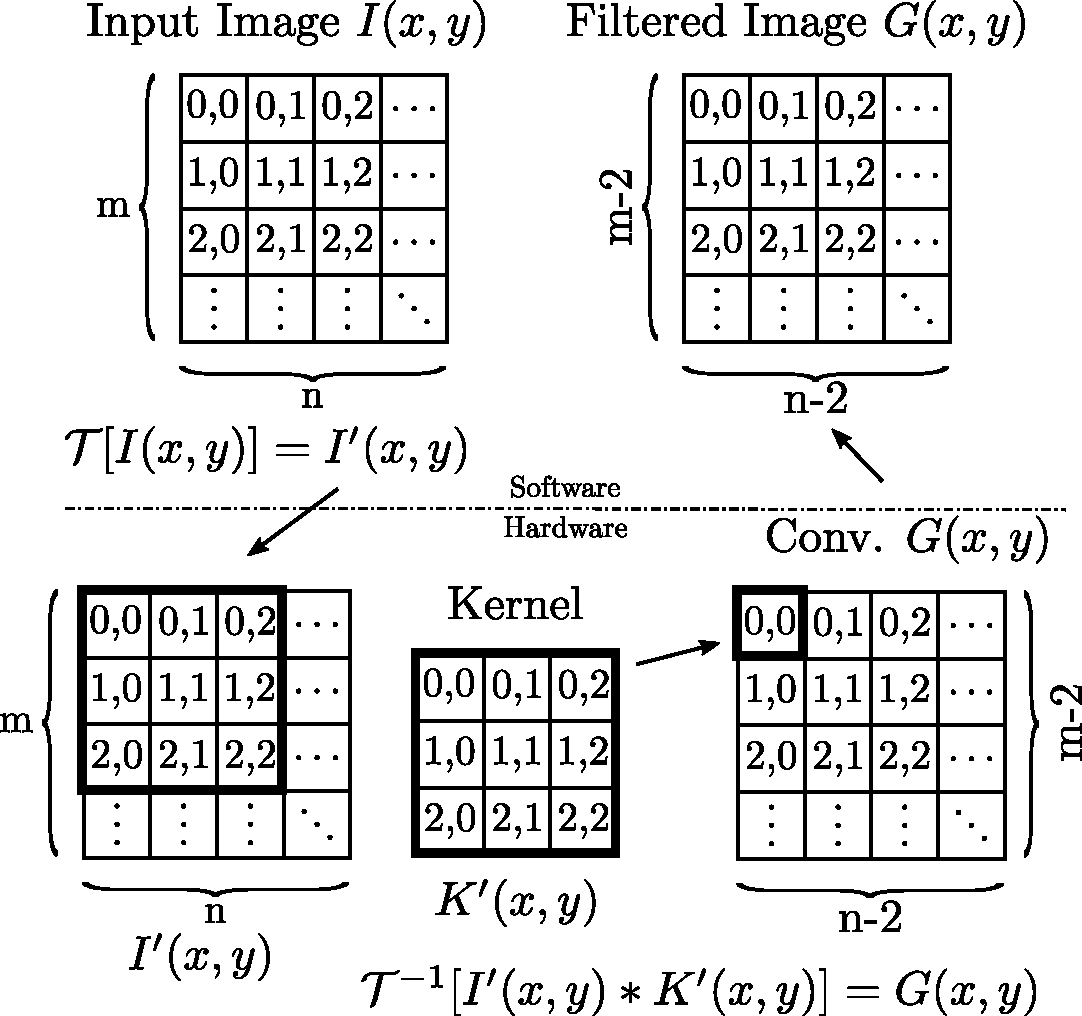
\includegraphics[scale=0.47]{wflow3}
\caption{Transformaciones del rango dinámico durante el procesamiento de la imagen.}
\label{transformation}
\end{figure}

\section{Representación en punto fijo}\label{fixedpoint}

La representación en punto flotante, almacena los números en términos de la
mantisa y del exponente. El hardware que soporta el formato punto flotante,
luego de ejecutar cada computo, automáticamente escala la mantisa y actualiza el
exponente para que el resultado se corresponda con el número de bits de forma
definida. Todas estas operaciones hacen que el hardware que soporte punto
flotante, sea más costoso en términos de área y potencia. Emerge una
alternativa: la representación en punto fijo.

La representación en punto fijo se emplea para
almacenar y manipular datos, con cierto número de bits fijos. Esto implica que
luego del cómputo, no se sigue la posición del punto decimal, y se le delega
esta responsabilidad al diseñador del hardware. El punto decimal, valga la
redundancia, es fijo para cada variable, y es predefinido. Fijando el punto, una
variable se limita a tomar un rango fijo de valores. Pese a que este límite nos
brinda ventajas en lo que refiere a utilización de recursos, si el resultado del
cómputo cae fuera del rango, se produce un overflow. Existen varias formas de
manipular los overflows que emergen como resultado de un cómputo en punto fijo
(redondeo, saturación, truncamiento) y sigue siendo responsabilidad del
diseñador optar por la representación adecuada según el sistema que pretende
llevar a cabo.

Este an\'alisis tiene por objeto el trabajar con una m\'inima representaci\'on
finita para los p\'ixeles de la imagen y los valores del kernel.
Para ello se necesita efectuar un estudio acerca de la cantidad de bits de
resoluci\'on m\'inimos  con una p\'erdida de informaci\'on aceptable.

Como se nombro anteriormente, los valores de los p\'ixeles \(I_{ij}\) se
encuentran en el rango 0 a 255. Con la normalización dynamic range
expansion se los lleva al rango 0 a 1. Los valores del kernel
\(K_{ij}\) pueden ser tanto positivos como negativos. Utilizando Maximum
norm se lleva al kernel al rango -1 a 1.

Para poder operar los rangos anteriores en una representaci\'on de 8 bits se
utiliza representac\'ion Signed Fixed Point\cite{fix_p} \(S(8,7)\). 

La convoluci\'on de una imagen con un $K^{3{\times}3}$ resulta en una 
salida de 20 bits, en \(S(16,14)\) por cada producto sumado la adici\'on de los nueve
elemento tiene una representaci\'on total de \(S(20,14)\).Entonces se realiza un
post procesamiento donde se lleva el resultado a un rango positivo y truncamiento.
Se establece una comparaci\'on a fines de decidir la cantidad de bits de salida del
procesamiento.

Para realizar una comparaci\'on se utiliza la relaci\'on SNR de la operaci\'on a
m\'axima resoluci\'on \(S(20,14)\) y el error producido al reducir la cantidad
de bits \(e_r=f(x)_{20b}-f(x)_{pos}\)\cite{srntesis}.

\begin{figure}
\centering
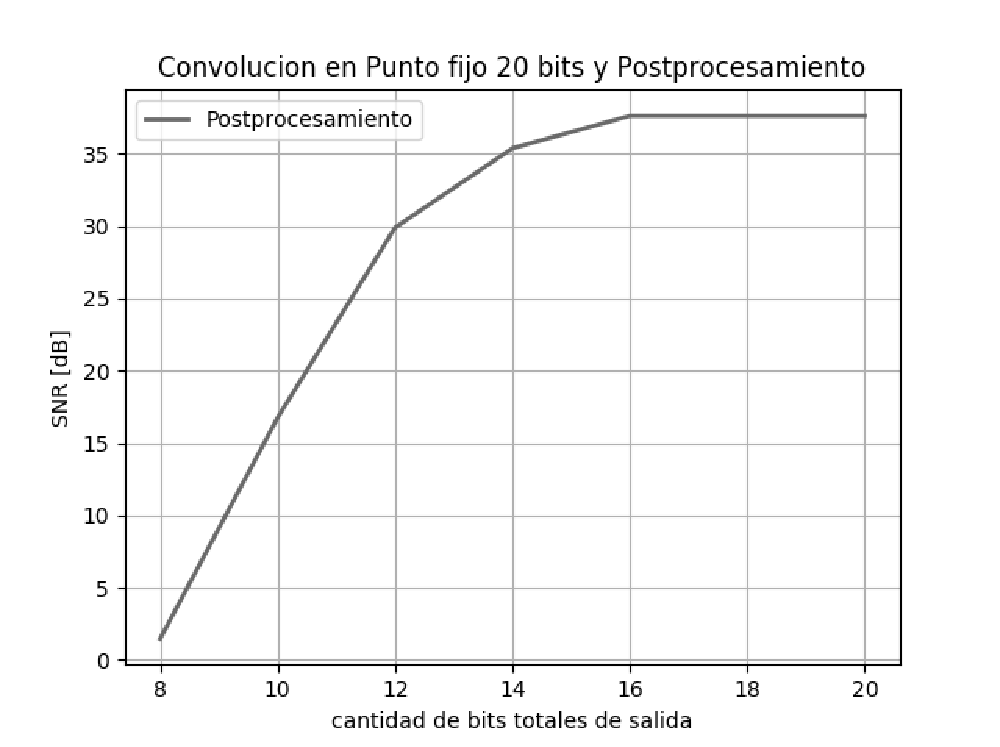
\includegraphics[scale=0.47]{posprocesamiento2}
\caption{Nivel de error según la resolución en bits.}
\label{prepro}
\end{figure}

Al la convolucionar con un filtro unitario y realizar una reducci\'on de los
bits de la parte fraccionaria, partiendo de 8 bits en totales, mejora la
representaci\'on de la imagen , y que a partir de 13 bits totales 1 bit de
signo, 5 bits parte entera y 7 en parte fraccionaria, con una representación
\(S(13,8)\) tiene una SNR aprimada de \(30 [dB]\) que permite observar el efecto
de la convolucion con una m\'inima perdida de informaci\'on recordando que
nuestro objetivo no es no es representar una imagen en su totalidad.

\begin{figure}[!t]
  \centering
  \subfloat{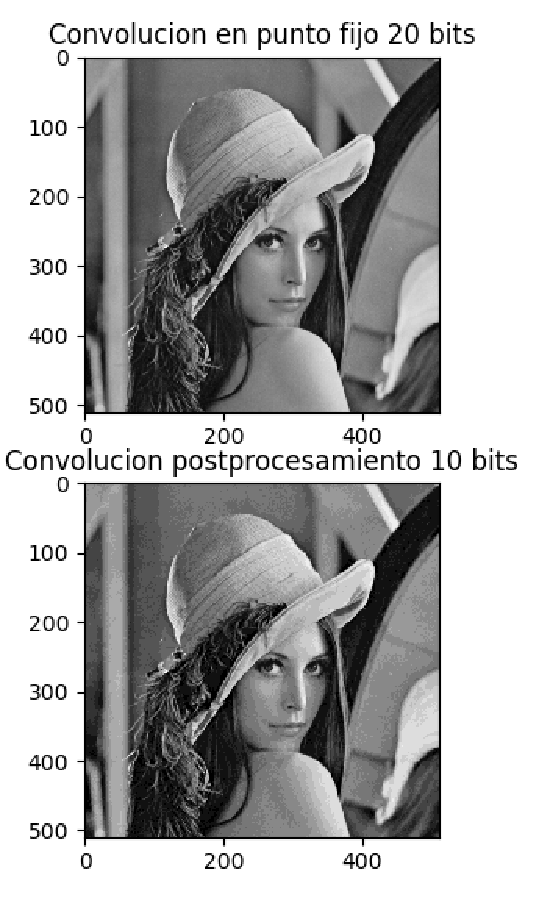
\includegraphics[scale=0.5]{posprocesanto1}}%
    \hfil %\vspace{0.1cm}
    \centering
    \subfloat{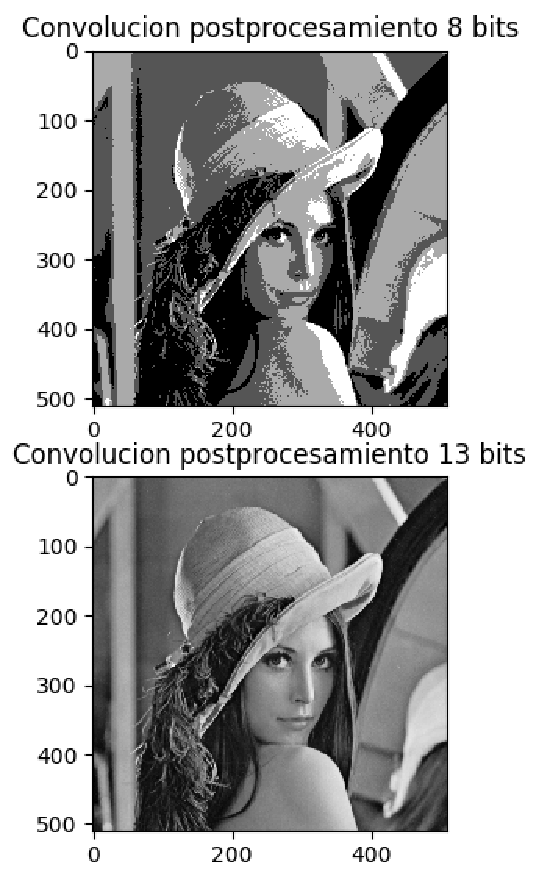
\includegraphics[scale=0.5]{posprocesanto2}}%
      \caption{Degradación de la imagen según la resolución en bits.}
      \label{prepro2}
    \end{figure}

Se puede llevar el rango final a 8 bits si se utiliza dynamic range expansion.
Pero se requiere conocer el m\'aximo y el m\'inimo valor de p\'ixel de la imagen
luego de filtrar, lo que implica que toda la imagen se encuentre en memoria.

\section{Flujo de diseño} \label{flujo_subsecc}

Se estructuró el proyecto y se siguió el flujo o estructura de la
Fig.~\ref{design_flow} para llevar el proyecto a cabo en el tiempo disponible.

En primera instancia se partió de las especificaciones, simulando el comportamiento en punto flotante mediante el lenguaje de alto nivel Python. Luego, se analizaron los resultados obtenidos tras implementar el sistema en punto fijo, a nivel software. 
Fijados los requerimientos se comenzó con el diseño del hardware,
previamente habiendo estudiado y modelado la arquitectura del sistema, la cual
se detalla en la seccion \ref{arquitectura_sec}.

\begin{figure}
\centering
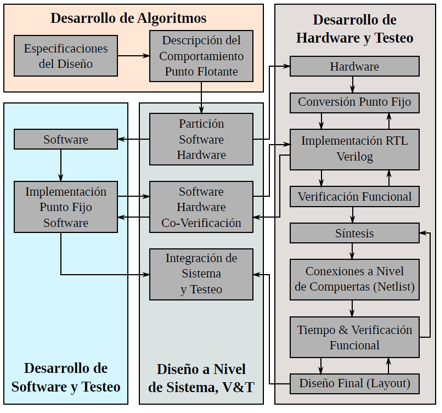
\includegraphics{flujo_de_dis.png}
\caption{Esquemático del flujo de diseño seguido.}
\label{design_flow}
\end{figure}

\subsection{Testing}

Se realizaron diferentes tipos de testing: test
unitarios de cada módulo (test bench del módulo), test de integración (varios
módulos y su interacción) y finalmente test de sistema, donde se probó el
funcionamiento del sistema completo dada cierta imagen de entrada. Para realizar
el proceso de testeo, en primera instancia se corrobora que los bits producidos
por el simulador del hardware descripto coincidieran con los bits del simulador
del sistema en Python, una vez pasada esta etapa con éxito, se implementa el
hardware en una FPGA y se comprueba nuevamente que los resultados obtenidos no
difieran con los simulados.

% \begin{figure}
% \centering
% 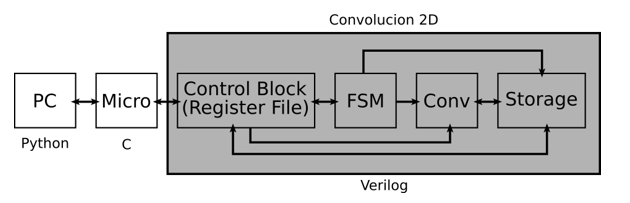
\includegraphics{general_sch.png}
% \caption{Diagrama general del sistema: comunicación y lenguajes empleados.}
% \label{general}
% \end{figure}
\chapter{Arquitectura del sistema}  \label{arquitectura_sec}
\section{Flujo de trabajo}  \label{workflow_subsecc}

Describiremos el diseño confeccionado en detalle. Se tienen tres etapas fundamentales:

\begin{itemize}
\item \textbf{Pre-procesamiento:} consiste en capturar la imagen aplicando las
  transformaciones mencionadas en la sección \ref{dynamicrange} y
  \ref{fixedpoint}, empleando un script hecho en Python. Este script divide la
  imagen en lotes o batches y los envía a la FPGA, a través del puerto UART. Un
  batch o lote, consiste en columnas contiguas de pixeles cuya dimensión se
  explica en la sección~\ref{storage_subsecc}.
\item \textbf{Procesamiento:}	: el batch es convolucionado con el kernel dentro del módulo. Dicho kernel es configurable, y el usuario puede cargar los coeficientes del mismo mediante el GPIO. 
  Cuando la operación de la convolucion finaliza, una notificación es enviada a
  un microprocesador en la FPGA, que da la orden de recuperar el batch procesado, para así enviarlo a la unidad central de procesamiento (CPU).
\item \textbf{Post-procesamiento:}Como etapa final, en el post-procesamiento se combinan los batches o lotes en CPU usando el script de Python.
\end{itemize}

\section{Estados y transiciones}  \label{states_subsecc}

\begin{figure}
\centering
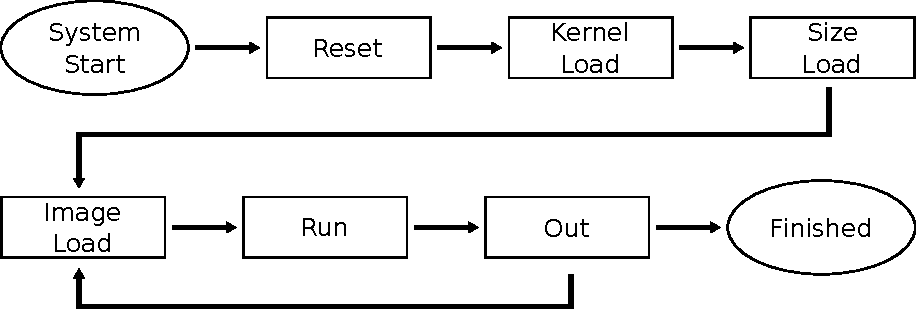
\includegraphics[scale=0.7]{states.pdf}
\caption{Diagrama de estados del sistema.}
\label{statesfig}
\end{figure}

El módulo atraviesa distintos estados para llevar a cabo su tarea. Estos estados
se pueden observar en la figura~\ref{statesfig}.

La transición entre un estado y
otro se realiza mediante instrucciones codificadas en el frame de entrada de 32
bits asentado en el GPIO. El módulo permanece en su estado actual hasta recibir
una instrucción valida.

Inicialmente, debe situarse al sistema en un estado de reset, y por ende debe
recibir una señal de reset para establecerse en dicho estado, esperando a ser
configurado.
Luego de recibir la correspondiente instrucción, se produce una transición hacia el estado KernelLoad, en donde los coeficientes del kernel se cargan al módulo.
El siguiente estado (SizeLoad), es en el cual se carga el tamaño de la imagen,
más precisamente la altura de la misma, esto permitirá conocer la posición del
último dato en memoria.
Estos tres estados mencionados, solo se ejecutan una vez durante todo el ciclo
de trabajo. El proceso se repite por cada nueva imagen, por ende, si se desea
procesar una nueva imagen, inicia el ciclo nuevamente.

Pasada la etapa de carga, la primera transición es hacia el
estado ImageLoad, donde se almacena el lote en la Block RAM de la FPGA.
Teniendo el lote almacenado, la transición luego es hacia el estado run donde se
hace el filtrado del lote, y mientras el sistema se situe en este estado, no
puede ser interrumpido.
Como consecuencia, cualquier instrucción recibida se ignora hasta que se
complete esta etapa de procesamiento de lote.

Cuando se finaliza el procesamiento de un lote, se emite una notificación y el sistema
queda en espera de la última señal para pasar hacia el estado Out. Una vez recibida la
correspondiente instrucción codificada, se devuelve el lote procesado al
microprocesador de la PC.

\begin{figure}
\centering
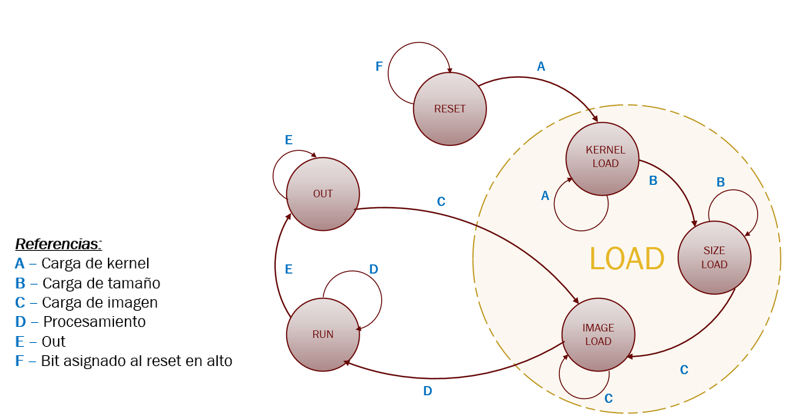
\includegraphics[scale=0.7]{states_2.png}
\caption{Diferentes estados y las etapas involucradas }
\label{statesfig2}
\end{figure}

\section{Arquitectura del módulo de convolución}  \label{ourdesign_subsecs}

El diseño planteado prioriza la reutilización dinámica de memoria, en donde por
cada iteración en la etapa de procesamiento, se aprovecha la disponibilidad de
datos cargados en memoria en la iteración anterior.
En la figura~\ref{general}, se muestran los bloques principales que conforman el
diseño. Los bloques que integran el módulo son:

\begin{figure}
\centering
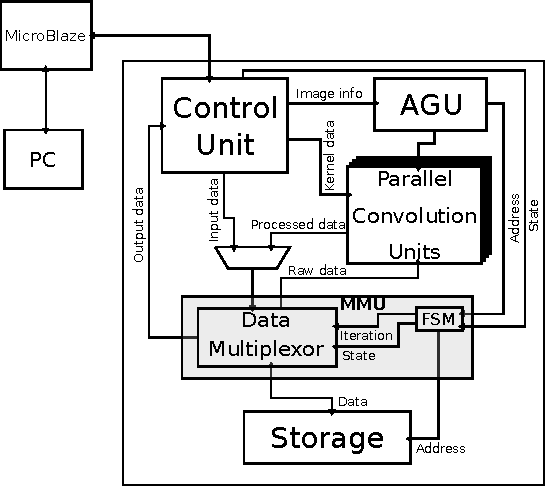
\includegraphics{general}
\caption{Arquitectura general del sistema }
\label{general}
\end{figure}

\begin{itemize}
\item \textbf{Control Unit:} se encarga del manejo de la comunicación entre el
  módulo y el procesador instanciado en la FPGA.\@
\item \textbf{MAC Unit -Multiplier-ACcumulator:} ejecuta la suma de los productos entre los coeficientes del kernel y los pixeles de la imagen. 
\item \textbf{Address Generation Unit (AGU):} bloque que maneja las direcciones
  de memoria que deben ser leídas o escritas.
\item \textbf{Memory Management Unit (MMU):} decide como son escritos y leídos
  los datos en la memoria.
\item \textbf{Storage:} hace referencia a un conjunto de columnas formadas por
  BRAMs de la FPGA.\@ El tamaño depende de la cantidad de MACs instanciadas,
  o en otras palabras, el paralelismo a nivel de cantidad de convoluciones en
  paralelo, que se desee en el sistema.
\end{itemize}
     
Estos bloques se describen en mas detalle en las secciones siguientes.

\subsection{Storage}\label{storage_subsecc}

Para almacenar un lote, se opto por organizar la BRAM en
columnas. Cada columna entonces, corresponde a una columna del lote.

El tamaño del lote está dado por la altura de la imagen y por el número de
columnas de memoria instanciadas.  La máxima altura en pixels de la imagen,
entonces, debe ser menor o igual al número de direcciones de una columna de
memoria instanciada.

Durante el procesamiento del lote, cada pixel se lee únicamente una vez, lo que
permite un uso mas eficiente de la memoria. Los pixeles del lote que ya fueron
leídos, se sobrescriben con los pixeles procesados. Esto permite reducir la
cantidad de memoria necesaria, ya que reúsa la misma memoria para almacenar el
lote de entrada, y el lote procesado.

Estas columnas de BRAM poseen dos puertos de direcciones y datos, uno para
los datos de entrada y otro para los datos de salida y además una señal de
control, write enable, que habilita la escritura de los datos de entrada en la memoria.

\subsection{Control Unit}\label{sec:ctrl_u}
El bloque Control Unit es el encargado de hacer de interfaz entre los bloques
restantes del módulo de convolución y el microprocesador que se encuentra en la
FPGA.\@ Para hacer esto, cuenta con dos puertos de 32 bits conectados a los GPIO
de entrada y salida del procesador.

El bloque interpreta las instrucciones que recibe y modifica las señales de
control conectadas a los otros bloques, esto representa la transición de
estados mencionada en la sección~\ref{states_subsecc}.

La organización del frame de entrada de 32 bits, junto con los códigos binarios
de las instrucciones se muestra en la tabla~\ref{instr}.

\begin{table}
% increase table row spacing, adjust to taste
\renewcommand{\arraystretch}{1.3}
% if using array.sty, it might be a good idea to tweak the value of
% \extrarowheight as needed to properly center the text within the cells
\caption{Código de instrucciones, la letra ``d'' representa bit de datos.}\label{instr}
\centering
% some packages, such as mdw tools, offer better commands for making tables
% than the plain latex2e tabular which is used here.
\begin{tabular}{|l|c|c|c|c|c|}
  \hline
  \multicolumn{1}{|c|}{\multirow{2}{*}{\textbf{Instrucción}}} & \multicolumn{5}{c|}{\textbf{BITS}} \\ \cline{2-6}
                                        & \textbf{31 - 29} & \textbf{28 - 25} & \textbf{24 - 14} & \textbf{13 - 1} & \textbf{0}\\\hline
  Cargar kernel                         & 000              & xxx              & ddddddddddd      & ddddddddddddd   & 0         \\\hline
  Cargar tamaño imagen                  & 001              & xxx              & xxxxxxxxxxx      & xxxdddddddddd   & 0         \\\hline
  Cargar lote                           & 010              & xxx              & xxxxxxxxxxx      & ddddddddddddd   & 0         \\\hline
  Recuperar dato                        & 011              & xxx              & xxxxxxxxxxx      & xxxxxxxxxxxxx   & 0         \\\hline
  Finalización de lote                  & 100              & xxx              & xxxxxxxxxxx      & ddddddddddddd   & 0         \\\hline
\end{tabular}           
\end{table}

Como el módulo y el procesador trabajan a distintas frecuencias de reloj, se
puede producir un error al enviar y recibir datos entre ambos. Para superar este
problema, el flanco ascendente del bit 28 se utiliza como indicador de que un
nuevo dato esta listo para ser leído o escrito. 

El bit 0 se utiliza como indicador del estado del módulo, en caso de ser 1 el
módulo se pone en estado de reset, por lo que una vez atravesado este estado,
siempre debería permanecer bajo.

Las instrucciones cumplen las siguientes funciones:

\begin{itemize}
\item \textbf{Cargar kernel:} Se utiliza para cargar los coeficientes del
  kernel, cada coeficiente es de 8 bits, junto con la instrucción se deben
  añadir los 3 coeficientes que forman una fila del kernel.\footnote{Para un
    diseño que utiliza kernels de $3\times3$, en caso de ser de dimensiones
    superiores, nuevas instrucciones deben ser añadidas.}
\item \textbf{Cargar tamaño imagen:} A esta instrucción debe acompañar el tamaño
  del alto en pixels de la imagen, se utilizan 10 bits para ello por lo que el
  tamaño máximo es de 1024px.
\item \textbf{Cargar lote:} Instrucción que indica que los datos corresponden a
  un pixel del lote.
\item \textbf{Finalización de lote:} Indica que el pixel que se esta cargando es
  el último pixel del lote, una vez recibida esta instrucción el módulo pasa al
  estado de run donde realiza el procesamiento.
\item \textbf{Recuperar dato:} Con esta instrucción se pide al módulo que
  entregue el pixel procesado siguiente.
\end{itemize}

Como se nombró anteriormente, una instrucción no será considerada hasta que no
haya un flanco ascendente en el bit 28.

\subsection{Address Generator Unit (AGU)}

El AGU es el encargado de generar las direcciones de memoria que son
consumidas por el MMU.

Durante el estado de ImageLoad, el AGU genera las direcciones donde se deben
escribir estos datos, para ello cuenta con un contador que se incrementa con
cada flanco de subida del bit 28 de la entrada del Control Unit
(sección~\ref{sec:ctrl_u}). El AGU además conoce el alto de la imagen (cargado
durante SizeLoad) por lo que una vez que el contador alcanza dicho valor envía
una señal al MMU indicando que el pixel que se recibe a continuación pertenece a
una nueva columna del lote.

Durante la etapa de procesamiento el AGU debe producir dos direcciones
diferentes, una que indica al MMU los datos que debe entregar a las unidades MAC
y otra que indica al MMU la posición donde los datos procesados por las MACs
deben ser almacenados. Ambas direcciones se incrementan una vez por ciclo de
reloj, pues las MAC generan un dato procesado por ciclo. La diferencia entre la
dirección de lectura y la dirección de escritura es igual a la latencia que
existe desde que se entrega el primer pixel a una unidad MAC hasta que el primer
pixel procesado este listo para almacenarse.

Durante el estado Out, o de salida de datos, el AGU genera las direcciones de
lectura de los datos procesados, al igual que en el estado de ImageLoad, se
incrementa con cada flanco de subida del bit 28 y tiene en cuenta el alto de la
imagen para hacer el cambio de columna de datos.

\subsection{Multiplier Accumulator Unit (MAC)}\label{sec:MAC}

Las MACs son unidades que se instancian en paralelo, son las encargadas de
hacer el calculo necesario para realizar la convolución. Poseen 9 registros
donde se almacenan los coeficientes del kernel y 9 registros donde se almacenan
los pixels de la porción del lote que se esta procesando en ese instante.

Las MAC poseen un único puerto de entrada de datos, donde se ingresan 3
coeficientes (correspondientes a una fila) del kernel o de una sección de lote
según le sea indicado por una señal proveniente del Control Unit. Además se
tiene otra señal de control donde se indica si los registros deben ser
modificados o permanecer congelados.

Para un kernel de tamaño $(k \times k)$, cada MAC Unit toma $k$ columnas de memoria
adyacentes como entrada. Se cargan entonces k pixeles de cada columna, quedando
$(k \times k)$ pixeles cargados dentro de ella, lo necesario para producir el
primer pixel procesado. Luego, se procede a efectuar la multiplicación de los
pixeles con los coeficientes del kernel y sumar cada termino. Al finalizar la
suma de los productos, el rango de los datos aumenta, por lo que antes de
ponerlos a la salida, las MAC realizan un truncado sobre los resultados.

\begin{figure}
\centering
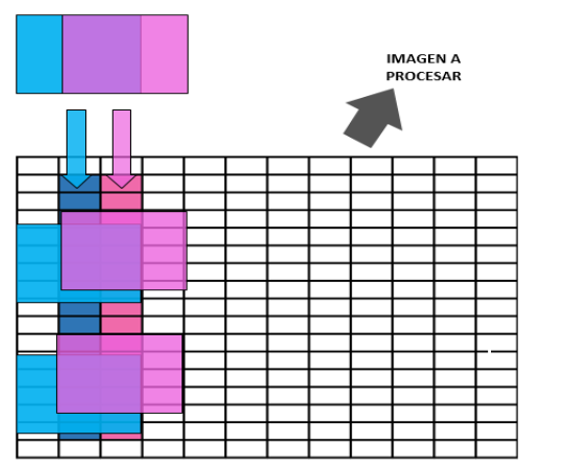
\includegraphics[scale=0.7]{conv1_despl.png}
\caption{Desplazamiento vertical del kernel sobre la imagen }
\label{verticaldesp}
\end{figure}

Una vez procesado un pixel, se efectua un desplazamiento (shift) de sus
registros en donde se almacenan pixeles del lote, para así descartar los $k$
pixeles mas antiguos, y se cargan los $k$ nuevos pixeles, es decir, una nueva
fila, lo que es equivalente a una estructura FIFO (First Input – First Output).
Se sincroniza lo mencionado anteriormente de forma tal de obtener un pixel
procesado por cada ciclo de reloj. Este procedimiento es equivalente a desplazar
verticalmente el kernel sobre la imagen como muestra la figura~\ref{verticaldesp}.

La estructura de hardware para realizar la operación se muestra en la figura~\ref{conv_struct},
como el hardware combinacional de los productos en cascada con la suma tiene un
tiempo de establecimiento de la salida mayor al período de reloj, se
introdujeron registros entre el hardware de los productos y la suma. Si bien
esto impacta en la latencia del bloque, la frecuencia de procesamiento se
mantiene en un pixel procesado por ciclo de reloj. 

\begin{figure}
\centering
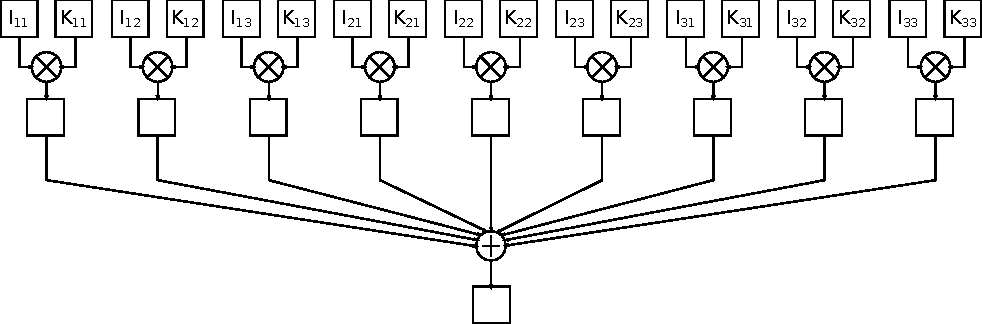
\includegraphics[scale=0.7]{conv_struct}
\caption{Estructura donde se realiza el calculo dentro de una unidad MAC.}
\label{conv_struct}
\end{figure}

\subsection{Memory Management Unit (MMU)}

Como se verá a continuación, para hacer un uso eficiente de las memorias es
necesario tener en cuenta el nivel de paralelismo. El objetivo del MMU es hacer
de interfaz entre las memorias y el resto de los bloques, independizándolos así del
nivel de paralelismo y reduciendo su complejidad.

En la sección~\ref{sec:MAC} se explicó que para un kernel de dimensión
$k \times k$ se necesitan $k$ columnas como entrada para producir una columna
procesada en una $MAC$ $Unit$. Por lo tanto, $2 \times k$ columnas, se necesitan
para $2$ $MACs$. Debido a la naturaleza de la operación de la convolución, para
obtener una columna contigua, se necesita desplazar una vez las columnas de
entrada. Entonces, existe un solapamiento entre las entradas de las MACs
que producen columnas adyacentes, y así la información puede ser compartida. 
Por esto, pese a necesitar $k$ columnas de entrada por cada unidad $MAC$,
solamente $k+1$ columnas diferentes de entrada se necesitan para dos $MACs$
instanciadas. Extendiendo este concepto a $N$ $MACs$, el número requerido de
columnas de memoria se reduce de $N \times k$ a $N+k-1$, concluyendo que
agregar una nueva unidad $MAC$ solamente agrega una nueva columna de memoria.

Debido al mismo solapamiento explicado anteriormente, hay información repetida entre
un lote recibido y el siguiente, por lo que, para reducir la transmisión de
datos, esta información repetida se mantiene en memoria y solamente se transmite
la parte faltante del lote entrante. Dadas $N$ $MACs$ y un kernel de $k \times k$,
un lote cuyo ancho (o cantidad de columnas) sea de $N+k-1$ es necesario. No
obstante, el lote procesado tendrá un ancho de  $N$ columnas, es decir, una por
unidad $MAC$, por lo que las ultimas $k+1$ memorias no se sobrescriben y
mantienen los datos de entrada. Estas $k+1$ columnas se reutilizan como las
primeras columnas del siguiente lote, y asi, el ancho del lote transmitido se
reduce a $N$, con la excepción de que el primer lote mantiene un ancho de
$N+k-1$.

La reutilización de columnas de memoria escritas por los lotes previos, resulta
en un desplazamiento circular en $N$ lugares, desplazando la posición de las
columnas de memoria asociadas con cada unidad $MAC$ en cada iteración. De lo
anterior, se deduce que existe una periodicidad entre la relación de columnas de
memoria y las entradas de las unidades $MAC$, donde el periodo $It$ es el número
de iteraciones necesario para obtener la relación ente las columnas de memoria
originales con respecto a las entradas de las unidades $MAC$. Matemáticamente
esto ocurre cuando $It$ es un múltiplo de $N+k-1$, esto es, debe existir un
número entero $m$, tal que:

\begin{equation}\label{niter}
  \frac{It}{m} = \frac{N}{k-1} + 1
\end{equation}

Comparado con un enfoque naive, donde cada MAC unit tendría sus $k$ columnas de
memoria independientes, el compartir información entre distintas MACs produce un
ahorro en el tamaño de BRAM necesaria, mientras que el desplazamiento circular
produce un ahorro en la cantidad de información transmitida. La
figura~\ref{comp} muestra una comparación de recursos utilizados por los
diferentes abordajes. Analizando la figura~\ref{transmitted} se observa que con el
abordaje naive es necesario transmitir casi 3 veces mas información (por ser un
kernel de $3 \times 3$) y no se ve afectado por el nivel de paralelismo.
En el caso de las entradas compartidas sin desplazamiento se tiene a disminuir
los datos redundantes transmitidos a medida que $N$ aumenta, esto es porque los
datos redundantes en un lote de $N+k-1$ es $k-1$ y $\frac{k-1}{N+k-1}$ tiende a
cero a medida que $N$ incrementa. El abordaje de las entradas compartidas con
desplazamiento circular es el caso óptimo donde no hay información redundante
transferida.

\begin{figure}%[!t]
\centering
\subfloat[][Cantidad de memoria requerida.]{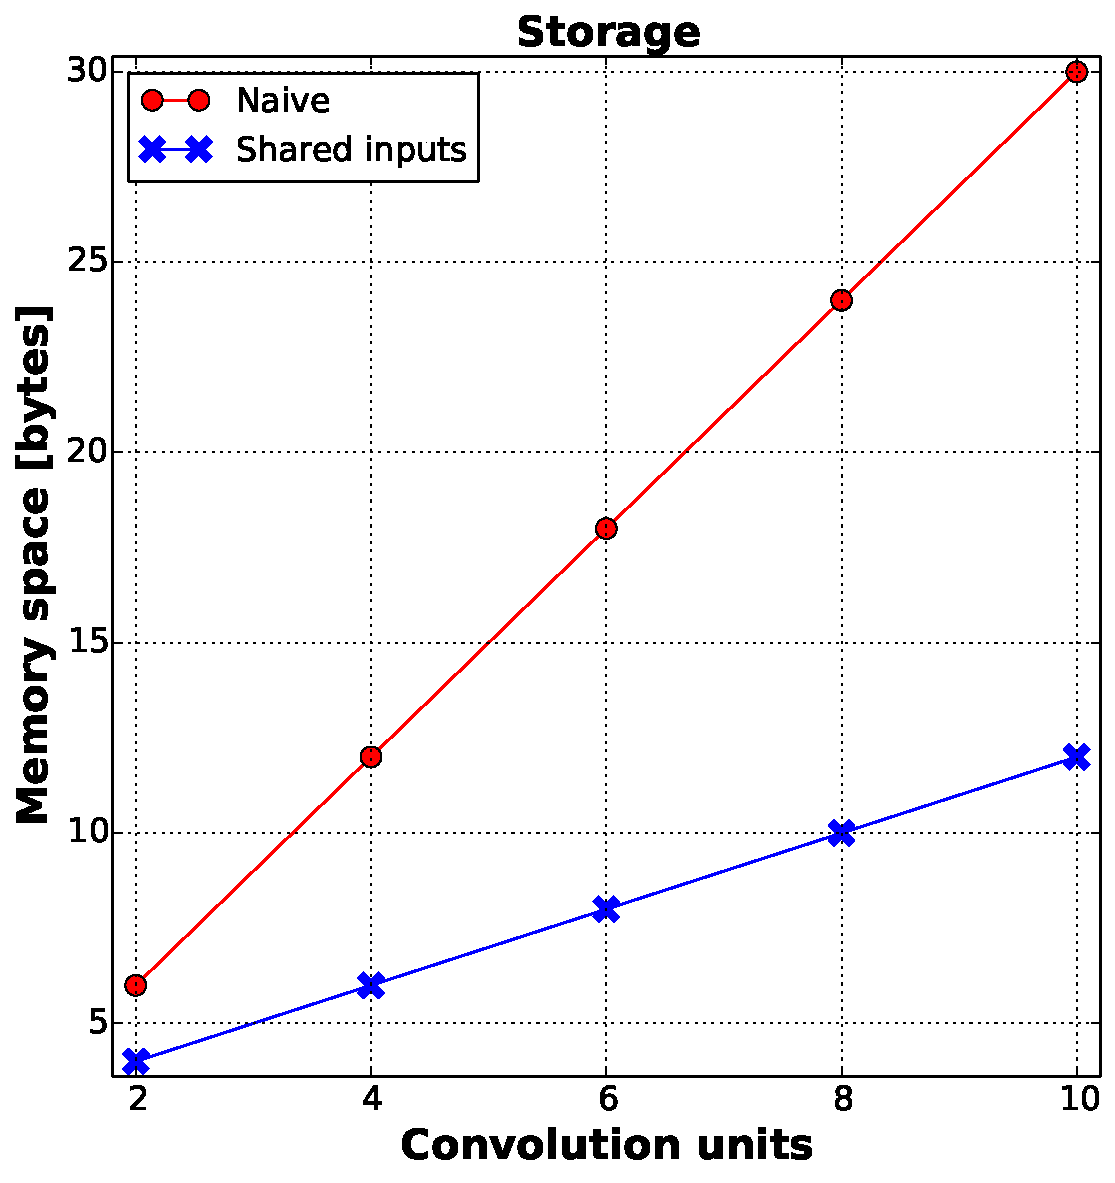
\includegraphics[scale=0.3]{mem_space2}%
\label{mem}}
\hfil %\vspace{0.1cm}
\centering
\subfloat[][Cantidad de datos transmitidos ]{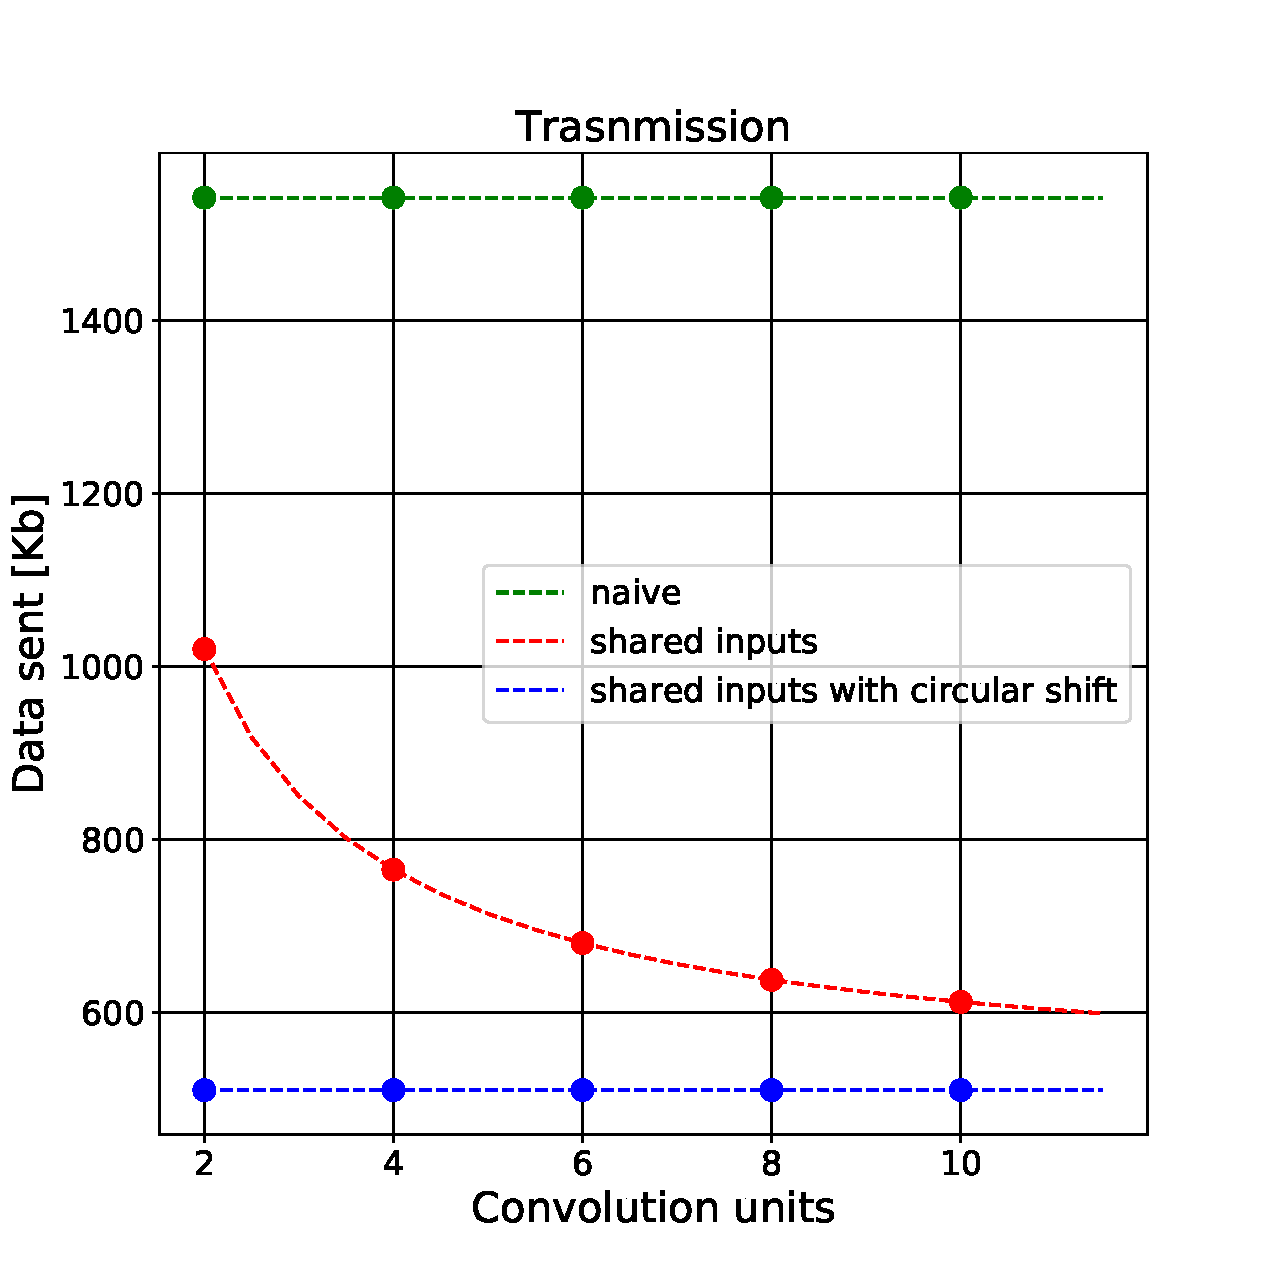
\includegraphics[scale=0.3]{data_sent}%
\label{transmitted}}
\caption{Comparación entre abordajes para una imagen de $1600\times1024$px y un kernel de $3\times3$.}\label{comp}
\end{figure}

Para asegurar un diseño escalable usando el abordaje de entradas compartidas con
desplazamiento circular, se concentró toda esta lógica en el MMU, simplificando
el diseño de los bloques restantes.

Este bloque, en cada iteración, mantiene un seguimiento de las posiciones de
memoria donde el lote entrante debe ser almacenado, la información que debe
alimentar a cada unidad MAC, las columnas de memoria donde la información
procesada debe ser almacenada y del orden en el cual la información procesada
debe ser devuelta.

Para cumplir con todas sus funciones, internamente el bloque se
compone de dos partes: una combinacional, llamada \textit{data multiplexer}, donde se
hace el encaminado de la información desde y hacia las memorias y las MACs, y
una parte secuencial basada en una máquina de estados finitos (FSM) que maneja
las señales de control de las memorias (write enable) y las señales de control
del data multiplexer.

\begin{table}
% increase table row spacing, adjust to taste
\renewcommand{\arraystretch}{1.3}
% if using array.sty, it might be a good idea to tweak the value of
% \extrarowheight as needed to properly center the text within the cells
\caption{Codificación de estados globales con las de señales SoP y EoP.}\label{MMU:glob_states}
\centering
% some packages, such as mdw tools, offer better commands for making tables
% than the plain latex2e tabular which is used here.
\begin{tabular}{|c|c|c|}
  \hline
  \textbf{Estado global} & \textbf{EoP} & \textbf{SoP}\\\hline
  Image Load             & 0            & 0           \\\hline
  Run                    & 1            & 0           \\\hline
  Out                    & 0            & 1           \\\hline
\end{tabular}           
\end{table}

El número de estados de la FSM esta dado por el número de iteraciones $It$ de la
ecuación~\ref{niter}. Cada estado de esta FSM interna representa una combinación de como se deben
escribir y leer los datos en las distintas columnas y no debe confundirse con
los estados globales del módulo explicados en la sección~\ref{states_subsecc}. Dichos
estados globales le son informados al MMU mediante dos señales de control:
comienzo de procesamiento (SoP) y fin de procesamiento (EoP). La
tabla~\ref{MMU:glob_states} muestra la codificación de dichas señales, se
observa que no están presentes todos los estados, esto es porque los estados
faltantes no afectan al comportamiento del MMU.\@ Además, el se cuenta con una
tercera señal, donde se informa que el siguiente dato debe ser escrito y leído
en la siguiente columna de memoria. 

El data multiplexer internamente se compone exclusivamente de multiplexores, que
pueden ser agrupados y clasificados en dos bloques más pequeños de acuerdo a la
función que cumplen: 

\begin{itemize}
 \item \textbf{$MMB$(Memory Multiplexer Blocks)}
  \item \textbf{$PMB$(Processing Multiplexer Blocks)}
\end{itemize}

La figura~\ref{mmu_routing} muestra el flujo de información entre unidades MAC,
MMU (data multiplexer) y las memorias. 
Los $MMB$ hacen el routing de la información sin procesar (raw data) y la
información desde las unidades $MAC$ hacia las memorias. 
Los $PMB$ hacen el routing de la información desde las memorias hacia las
unidades $MAC$. La figura~\ref{mmu_structure} muestra como están formados ambos
bloques.

\begin{figure}
\centering
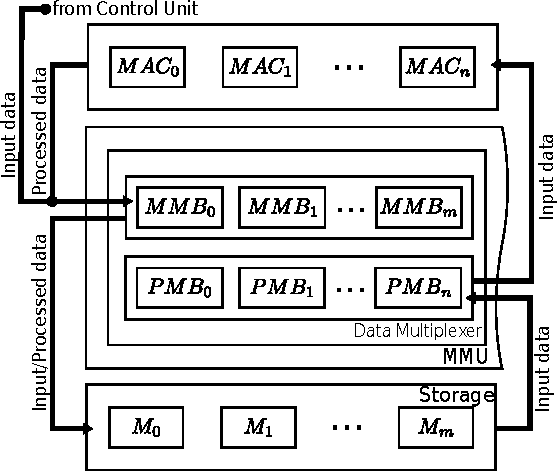
\includegraphics[scale=0.9]{muxes}
\caption{Enrutamiento de información}\label{mmu_routing}
\end{figure}

\begin{figure}
\centering
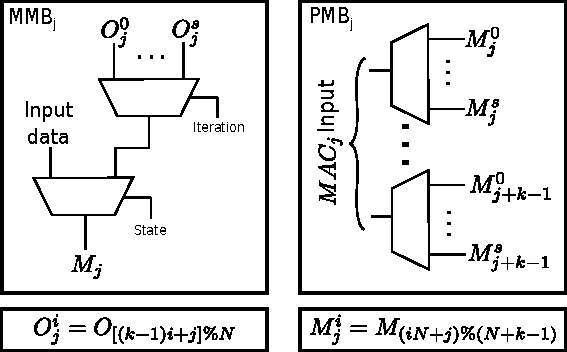
\includegraphics{muxes_cont}
\caption{Estructura de los bloques MMB y PMB.}\label{mmu_structure}
\end{figure}

Tanto los bloques $MMB$ como los $PMB$ tienen un numero de entradas proporcional
al numero de estados de la $FSM$ interna del bloque $MMU$. Las entradas
a sus multiplexores se definen respectivamente: 
\begin{equation}%\label{niter}
  O_j^i = O_{[(k-1)i+j]\%N}
\end{equation}
\begin{equation}%\label{niter}
  M_j^i = M_{(iN+j)\%(N+k-1)}
\end{equation}
donde el símbolo $ \% $ representa la operación módulo, e $i$ toma valores desde
$0$ a $It-1$.
\chapter{Implementación y resultados}  \label{implementations_sec}

\section{Especificaciones}

El diseño fue implementado en una FPGA Xilinx Artix-35T (xc7a35ticsg324-1L)
utilizando las herramientas del software Xilinx Vivado Design Suite 2017.4. Se
trabajó con un clock de referencia de $100$ MHz, y el script para el
pre-procesamiento y el post-procesamiento fueron escritos en Python 2.7. 

Tanto los coeficientes del kernel como el correspondiente lote de imagen, se
cargan a la placa a través del puerto UART. Si bien esta vía es lenta con
respecto al tiempo de procesamiento, se optó por utilizarla debido a su
simplicidad y al bajo consumo de recursos comparado a otros medios de
transmisión.

En lo que refiere a representación de datos, como se explica en la
sección~\ref{fixedpoint}, se trabajó con aritmética en punto fijo, con una
resolución de $U(8,0)$ para la imagen de entrada y salida (imagen procesada), y
$S(8,7)$ para el kernel.

\section{Verificación}

Para verificar el comportamiento del sistema. se armaron diferentes kernels
en Python, y se aplicaron los mismos a una imagen de prueba. Luego, 
se filtró a la imagen con los mismos kernels  pero utilizando la FPGA
Los kernels que se utilizaron fueron: identidad $[0, 0, 0; 0, 1, 0; 0, 0,
0]$ sharpening $[0, -1, 0; -1, 5, -1; 0, -1, 0]$ y embossing $[-2, -1, 0; -1,
0, 1; 0, 1, 2]$. La figura~\ref{images_py_po} los resultados obtenidos.

\begin{figure}[!t]
\centering
\subfloat[][Identidad]{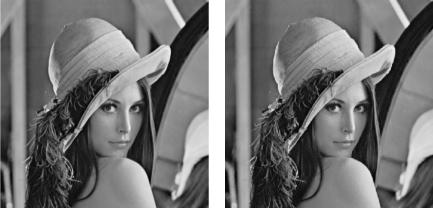
\includegraphics[scale=1.1]{identity_c}
  \label{fig:identity}}
\hfil
\subfloat[][Sharpening]{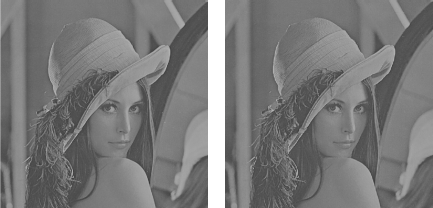
\includegraphics[scale=1.1]{shaped_c}
  \label{fig:share}}
\hfil
\subfloat[][Embossing]{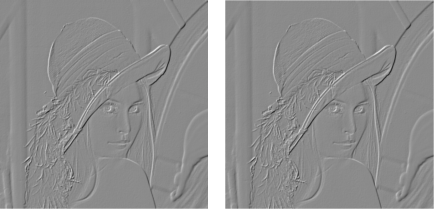
\includegraphics[scale=1.1]{emboss_c2}
\label{fig:embossing}}
\caption{Comparación de resultados: A la izquierda, la imagen procesada en una CPU usando python y, a la
  izquierda, la misma imagen procesada con el módulo en la FPGA.}
\label{images_py_po}
\end{figure}

\section{Utilización de recursos}

La arquitectura se sintetizó para diferentes grados de paralelismo. La tabla
Tabla~\ref{res_table} muestra la complejidad del módulo y el microprocesador en
la FPGA con y sin el uso de DSP respectivamente, medida por la utilización de
recursos. Se ve un incremento lineal acorde al grado de paralelismo en el
sistema. Debido a las limitaciones de la FPGA utilizada, se llegó a instanciar
$8$ $MAC$ $units$ para que operen en pparalelo con DSP, y $24$ sin el uso de DSP
pero con una utilización de $LUTs$ más intensiva.

\begin{table}
% increase table row spacing, adjust to taste
\renewcommand{\arraystretch}{1.3}
% if using array.sty, it might be a good idea to tweak the value of
% \extrarowheight as needed to properly center the text within the cells
\caption{Utilización de recursos con y sin DSP.}
\label{res_table}
\centering
% some packages, such as mdw tools, offer better commands for making tables
% than the plain latex2e tabular which is used here.
\begin{tabular}{|c|c|c|c|c|c|c|}
  \hline
  & \multicolumn{3}{c|}{\textbf{With DSP [N](\%)}} & \multicolumn{3}{c|}{\textbf{Without DSP [N](\%)}} \\ \hline
  \textbf{P}  & \textbf{DSP}            & \textbf{LUT}        & \textbf{BRAM}       & \textbf{DSP}         & \textbf{LUT}           & \textbf{BRAM}         \\ \hline
  2  & 20(22)         & 1845(9)    & 10(20)     & ---         & 3168(15)      & 10(20)         \\ \hline
  4  & 40(44)         & 2022(10)   & 11(22)     & ---         & 4627(22)      & 11(22)         \\ \hline
  6  & 60(67)         & 2175(10)   & 12(24)     & ---         & 6063(29)      & 12(24)         \\ \hline
  8  & 80(89)         & 2448(12)   & 13(26)     & ---         & 7756(37)      & 13(26)         \\ \hline
  10 & ---            & ---        & ---        & ---         & 9328(45)      & 14(28)         \\ \hline
  12 & ---            & ---        & ---        & ---         & 10917(52)     & 15(30)         \\ \hline
  24 & ---            & ---        & ---        & ---         & 20209(97)     & 21(42)         \\ \hline
\end{tabular}           
\end{table}

También se realizó una comparación, mostrada en la figura~\ref{bram_n}, entre la
utilización de BRAM estimada, y los resultados obtenidos de la síntesis. Se
efectuó una normalización con respecto al porcentaje de utilización de BRAM
dividiendo el máximo valor de porcentaje de utilización, y considerando que la
instancia del microblaze ya ocupa $18\%$ de los recursos BRAM.
Puede observarse que el comportamiento lineal anticipado por los
cálculos teóricos, es consistente con los resultados de la síntesis.

\begin{figure}
\centering
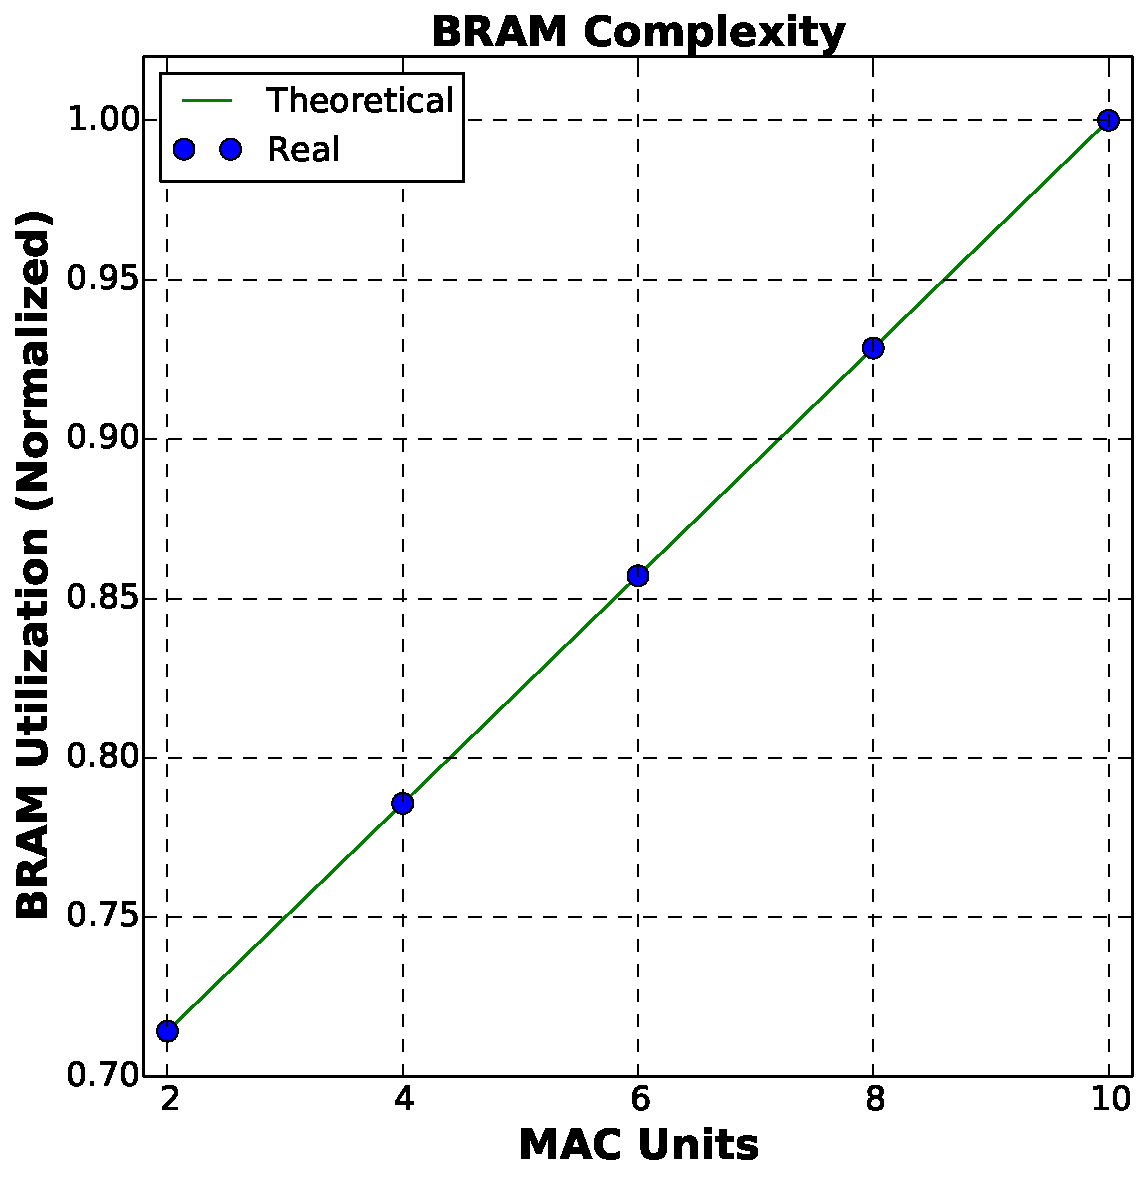
\includegraphics[scale=0.3]{BRAM_c2}
\caption{Curva normalizada para la utilización de los recursos de BRAM.}
\label{bram_n}
\end{figure}

\section{Throughput}

Considerando únicamente la operación de convolución, es decir, no teniendo en
cuenta el tiempo necesario para cargar la imagen en memoria, se obtiene un pixel
por ciclo de clock ($100$ Mhz) por cada $MAC$ $Unit$ instanciada. 

El throughput incrementa linealmente con el grado de paralelismo. La tabla
\ref{conv_tp} muestra el throughput obtenido para los diferentes grados de
paralelismo.

\begin{table}
% increase table row spacing, adjust to taste
\renewcommand{\arraystretch}{1.3}
% if using array.sty, it might be a good idea to tweak the value of
% \extrarowheight as needed to properly center the text within the cells
\caption{Throughput obtenido en lo que respecta a la convolución.}
\label{conv_tp}
\centering
% some packages, such as mdw tools, offer better commands for making tables
% than the plain latex2e tabular which is used here.
\begin{tabular}{|c|c|c|}
 \hline
  \textbf{Parallelism}  &    \textbf{Processing Speed [Mp/s]}  \\ \hline
          2             &                     200              \\ \hline
          4             &                     400              \\ \hline
          8             &                     800              \\ \hline
\end{tabular}           
\end{table}
%TODO: añadir appa
%% This defines the bibliography file (main.bib) and the bibliography style.
%% If you want to create a bibliography file by hand, change the contents of
%% this file to a `thebibliography' environment.  For more information 
%% see section 4.3 of the LaTeX manual.
\begin{singlespace}
\bibliography{main}
\bibliographystyle{plain}
\end{singlespace}

% TODO: añadir las referencias en la biblografia
\end{document}

